\documentclass[10pt, landscape, a4paper]{article}
\usepackage{geometry}[landscape]
\usepackage{multicol}
\usepackage{graphicx}
\usepackage{amsmath} 
\usepackage{amssymb}
\usepackage{ccicons}
\usepackage{hyperref}

\usepackage[dvipsnames]{xcolor}

% Set page margins
\geometry{top=.8cm, left=.8cm, right=.8cm, bottom=.8cm}

% Set paragraph indentation
\setlength{\parindent}{0pt}

% Set path for assets
\graphicspath{{assets/}}

\setlength{\columnsep}{20pt}
\raggedcolumns

% _____ CUSTOM COMMANDS __________________________________________
\newcommand{\E}[0]{\mathbb{E}}
\newcommand{\R}[0]{\mathbb{R}}

\newcommand{\sgn}[0]{\text{sgn}}

\newcommand{\argmin}[1]{\underset{#1}{\text{argmin}}}
\newcommand{\argmax}[1]{\underset{#1}{\text{argmax}}}

\begin{document}
\begin{multicols*}{3}

% _____ CONTENT __________________________________________________

% main heading
\begin{center}
	\Large{\textbf{Computer Systems}} \\
    \small{by dcamenisch}
\end{center}

\section{Introduction}

asdfhkajdsfhasöj

\section{Naming}

Naming is a fundamental concept, it allows resources to be bound at different times. Names are bound to objects, this is always relative to a context. One example of this would be path names, e.g. \textit{/usr/bin/emacs}. Name resolution can be seen as a function from context and name to some object. The resolved object can be a context in itself. This gives us a naming network.
\begin{center}
	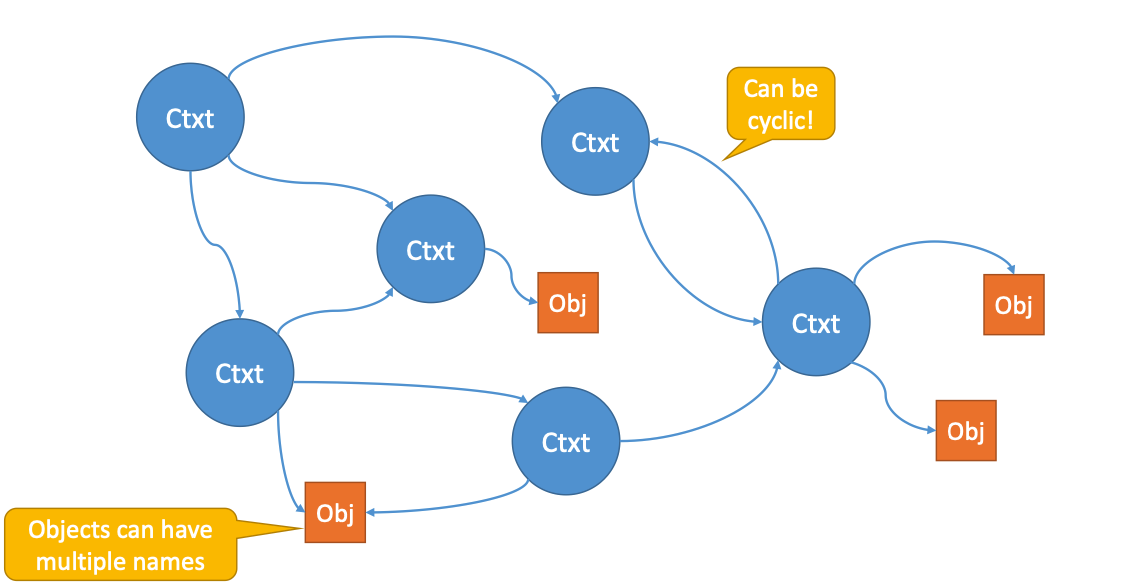
\includegraphics[width=0.8\linewidth]{naming-network.png}
\end{center}

Both synonyms (two names bound to the same object) and homonyms (the same name bound to two different object) can occure.

\end{multicols*}
\end{document}

% ____ FOOTER ______________________________________________________
% Content and Template: 
% original by Danny Camenisch (dcamenisch@inf.ethz.ch), 2022
% based on different summaries from many helpful people